\documentclass{deimj}
\usepackage{graphicx}
\usepackage{listings,jlisting}
%\usepackage{latexsym}
%\usepackage{txfonts}
%\usepackage[fleqn]{amsmath}
%\usepackage[psamsfonts]{amssymb}
%\usepackage[deluxe]{otf}

% 印刷位置調整 %
% 必要に応じて値を変更してください.
\hoffset -10mm % <-- 左に 10mm 移動
\voffset -10mm % <-- 上に 10mm 移動

\lstdefinelanguage{JavaScript}{
  keywords={typeof, new, true, false, catch, function, return, null, catch, switch, var, if, in, while, do, else, case, break},
  keywordstyle=\color{blue}\bfseries,
  ndkeywords={class, export, boolean, throw, implements, import, this},
  ndkeywordstyle=\color{darkgray}\bfseries,
  identifierstyle=\color{black},
  sensitive=false,
  comment=[l]{//},
  morecomment=[s]{/*}{*/},
  commentstyle=\color{purple}\ttfamily,
  stringstyle=\color{red}\ttfamily,
  morestring=[b]',
  morestring=[b]"
}


\lstset{%
  language=JavaScript,
  basicstyle={\small},%
  identifierstyle={\small},%
  commentstyle={\small\itshape},%
  keywordstyle={\small\bfseries},%
  ndkeywordstyle={\small},%
  stringstyle={\small\ttfamily},
  frame={},
  breaklines=true,
  columns=[l]{fullflexible},%
  numbers=left,%
  xrightmargin=0zw,%
  xleftmargin=3zw,%
  numberstyle={\scriptsize},%
  stepnumber=1,
  numbersep=1zw,%
  lineskip=-1ex%
}

\newcommand{\AmSLaTeX}{%
 $\mathcal A$\lower.4ex\hbox{$\!\mathcal M\!$}$\mathcal S$-\LaTeX}
\newcommand{\PS}{{\scshape Post\-Script}}
\def\BibTeX{{\rmfamily B\kern-.05em{\scshape i\kern-.025em b}\kern-.08em
 T\kern-.1667em\lower.7ex\hbox{E}\kern-.125em X}}

\papernumber{DEIM Forum 2014 XX-Y}

\jtitle{実世界プログラミングのための分散人力処理環境}
\jsubtitle{}
\authorlist{%
 \authorentry[bb@sfc.keio.ac.jp]{馬場 匠見}{Takumi BABA}{Keio}% 
 \authorentry[shokai@sfc.keio.ac.jp]{橋本 翔}{Sho HASHIMOTO}{Keio}% 
 \authorentry[masui@pitecan.com]{増井 俊之}{Toshiyuki MASUI}{Keio-Faculty}% 
}
\affiliate[Keio]{慶應義塾大学政策・メディア研究科\hskip1zw
  〒252-0882 神奈川県藤沢市遠藤5322}
 {Graduate School of Media and Governance,
  Keio University\\
  5322 Endo, Fujisawa,
  Kanagawa 252-0882, Japan}
\affiliate[Keio-Faculty]{慶應義塾大学環境情報学部\hskip1zw
  〒252-0882 神奈川県藤沢市遠藤5322}
 {Faculty of Environment and Information Studies,
   Keio University\\
  5322 Endo, Fujisawa,
  Kanagawa 252-8520, Japan}  

%\MailAddress{$\dagger$hanako@deim.ac.jp,
% $\dagger\dagger$\{taro,jiro\}@jforum.co.jp}

\begin{document}
\pagestyle{empty}
\begin{jabstract}
本論文では、プログラム上で人の行動を記述するためのプログラミング環境 BabaScript を提案する。
コンピュータの動作の手順書としてプログラムが、人間の行動の手順書としてマニュアルやレシピといったものが存在するが、両者を同一のフォーマットで記述することはできない。
BabaScriptは、人への命令構文と値を返すことのできるクライアントアプリケーションを組み合わせることで実現する、人の行動をプログラムに記述可能にするプログラミング環境だ。
BabaScript環境によって、人・実世界・コンピュータの世界をより柔軟にプログラムすることが可能になる。
\end{jabstract}
\begin{jkeyword}
ヒューマンコンピュテーション, プログラミング環境, 実世界プログラミング
\end{jkeyword}
\maketitle

\section{はじめに}

コンピュータの動作を制御するための手順書としてプログラムが存在する。
このプログラムを実行することによって、様々な計算が可能となっている。
近年では、実世界をプログラミングするために、センサ・アクチュエータを利用するようになっており、プログラムが記述できる処理は増え続けている。

人間の動作を制御するための手順書としては、レシピであったりマニュアルといったものが存在する。
手順書に従うことによって、人間は適切・効率的に動作し、目的を達成できる。
レシピやマニュアルの中身は、プログラムと同じようなものである。
人に実行させたい処理が記述されており、人は記述内容を自分で解釈し、実行していく。
例えば、プログラム風に書くと、料理のレシピには

\begin{lstlisting}[caption=,label=]
if 鍋の水が沸騰する == true
  パスタを鍋に投入する
\end{lstlisting}
    
というようなことが、小売店の店員マニュアルには

\begin{lstlisting}[caption=,label=]
if レジに人が並んでいる == true
  2番レジを開ける
\end{lstlisting}
    
といった記述がされており、内容は人によって実行されている。

プログラムとレシピやマニュアルは、実行手順を表すという意味では同じものであるが、別の存在として認識されており、同一のフォーマット上で記述することはできない。
一方、近年の研究では、プログラム中に計算資源として人を使うといった提案もなされている。
両者の壁は取り払われつつあるが、人とコンピュータ、両方の世界を記述するための統一的な記述法は存在しない。

本論文では、人の行動をプログラム内に記述可能なプログラミング環境 BabaScript を提案する。
BabaScript環境によって、人の行動をプログラム内で記述可能となり、同一フォーマット上で人とコンピュータ両方への命令を記述することができる。
また、特殊なプログラミング言語を使わず、高い拡張性を持つため、様々なアプリケーションに組み込むことができる。

\section{BabaScript}

BabaScriptは、人への命令構文をプログラミング言語に付加するライブラリと、プログラムからの命令を受け取り、処理結果をプログラムに返すクライアントライブラリを組み合わせることで実現するプログラミング環境だ。
BabaScript環境下では、プログラム内で人への命令が記述可能となる。
どちらのライブラリも、簡単に拡張・組み込みが可能となっており、既存のアプリケーションでも簡単にBabaScript環境を導入することができる。

\subsection{人への命令構文}
人への命令構文を含んだオブジェクト(以下、人オブジェクト)を宣言可能にするライブラリを実装した。
人オブジェクトを宣言し、そのオブジェクトのメソッドを実行をすることで、人への命令が可能となる。
オブジェクトに定義されていないメソッドは全て人への命令として解釈され、メソッドと引数を元に人への命令内容が生成される。
例えば、以下のサンプルで示しているような日本語メソッドは基本的に定義されていないため、人への命令として解釈される。

プログラム内で人オブジェクトを宣言するときには、第一引数にidを指定する。
このidと同一のidを持つクライアントに対し、命令の配信が行われる。
また、複数のクライアントアプリケーションが同一のidによって生成されている場合、特別なオプションがない場合は、命令は各クライアントアプリケーションに分散して配信される。
以下のプログラムのような記述方法によって、人オブジェクトを宣言し、人に対して命令を送ることができる。

\begin{lstlisting}[caption=,label=]
baba = new Baba.Script("baba");
baba.書類整理をする({num: 5}, function(result){
  ...
});
\end{lstlisting}
上記のプログラムの場合、メソッド名である"書類整理をする"と第一引数である "{num: 5}" が命令としてクライアントアプリケーションに通知される。

人への命令メソッドの第一引数にオブジェクトを与えることによってクライアントアプリケーション側にオプションとして情報を送ることができる。
特別なオプションとしてbroadcast が存在する。

\begin{lstlisting}[caption=,label=]
baba.大学内にいますか({broadcast: 5}, function(result){ ... });
\end{lstlisting}

上記のように、オプションに broadcast: num を指定することによって、同じidを持つ全クライアントに対して同様の命令を送信し、 num で指定した数だけ値が返ってきたらコールバック関数を実行することができる。

オプションの例としては返り値の型指定がある。
プログラムへの返り値として様々な型が考えられるが、全ての型を考慮してプログラムを記述することは難しい。
返り値の型を指定することによって、プログラム側で求めている値を人に入力させることが可能だ。
数値の返り値を求める場合であれば、以下のようなプログラムを書き、クライアントアプリケーション側で数値だけを入力させるインタフェースを表示させるといったことが考えられる。

\begin{lstlisting}[caption=,label=]
baba.部屋の中には人が何人いますか({format: "int"}, function(result){ ... });
\end{lstlisting}
数値の他にも、文字列であったりリストの中から選択する、といったフォーマットが考えられる。

\subsection{クライアント}

命令を受け取り、値をプログラムに返すための一連の機能をクライアント側のライブラリとして実装した。
javascript,objective-c,java の3言語で実装されており、iOSやandroidなどのモバイルデバイス上のアプリケーションで利用することを想定している。
クライアント側では、BabaScript通信用のクライアントオブジェクトを宣言し、このオブジェクトを通すことでプログラム側との通信が可能となる。
このクライアントオブジェクトからのメッセージを受け取る関数を実装することによって、プログラマ側で自由にクライアントアプリケーションを実装できる。
以下のようなプログラムで、人への命令構文を用いたプログラムからのメッセージを受け取ることができる。

\begin{lstlisting}[caption=,label=]
client = Baba.createClient("baba");
client.on("get_task", function(order){
  #プログラムからメッセージを受け取った時の挙動を記述する
});
\end{lstlisting}

メッセージを受け取る関数内において、ユーザに命令を伝え、処理結果を入力するようなインタフェースを生成してワーカーに提示する必要がある。
また、クライアントオブジェクトが持つメソッド returnValue を使うことで、プログラムに処理結果を返すことができる。
以下のようなプログラムが考えられる。

\begin{lstlisting}[caption=,label=] 
client.on("get_task", function(result){
  order = new Order(result.key)
  input = new Input(result.format)
  input.on("submit", function(value){
    client.returnValue(value)
  });  
});
\end{lstlisting}

  
\subsection{人への命令構文実行時の流れ}
BabaScript環境では、以下のような流れで人への命令が配信され、返り値を得ることができる。

\begin{enumerate}
\item プログラムで人への命令構文を実行する
\item ネットワークを介して、適切なBabaScript Clientに命令が配信される
\item BabaScript Client は、命令をユーザに通知する
\item 人が命令を処理する
\item 人は処理結果をBabaScript Clientに入力する
\item 結果をネットワークを介して、プログラムに返す
\item プログラムは、返ってきた値を元に指定された続きの処理を実行する
\end{enumerate}

システムの全体図を以下に示す

\begin{figure}[tb]
  \begin{center}
    \fbox{
      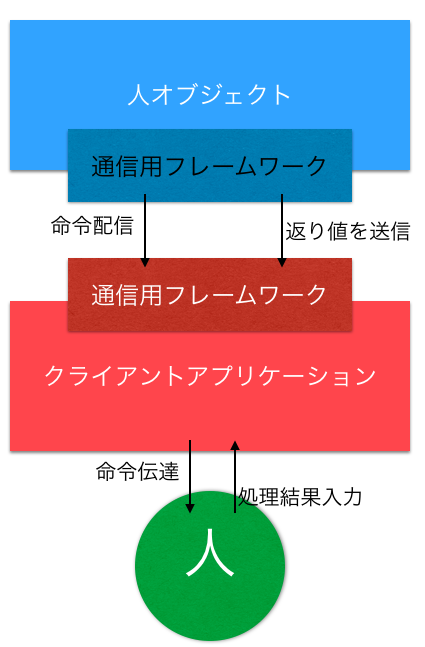
\includegraphics[width=40mm, bb = 0 0 425 647]{images/framework-image.png}
    }
    \caption{システム図}
    \label{system}
  \end{center}
\end{figure}



\subsection{特徴}
\subsubsection{オブジェクトとして人を表現可能}
普通にプログラムを書いている中で、オブジェクトを扱っているのと同じような手法で人オブジェクトを利用可能である。
人オブジェクトのメソッドを実行すれば、普通のオブジェクトと同じように値が返ってくるため、普通のプログラム記述の手法で人の行動をプログラムすることができる。

\subsubsection{アプリに人力処理を組み込む}
クライアント用のライブラリを読み込み、クライアントオブジェクトを生成するだけで、どんなアプリ上でも人力処理のワーカーになることができる。
拡張性がとても高く、既存のアプリケーションにも組み込むことができる。

\subsection{サンプル}
例えば、パスタ料理をつくるプログラムならば、以下のプログラム群のような記述方法が考えられる。

\subsubsection{人への命令を記述したプログラム}
人への命令を記述するプログラムは、以下のようなものが考えられる。

\begin{lstlisting}[caption=,label=]
  baba = new Baba.Script("takumibaba")
  list = ["ペペロンチーノ", "カルボナーラ", "トマトクリーム", "ボロネーゼ"]
  baba.どれを作りますか({format: "list", list: list}, function(data){
    if(data.value === "ペペロンチーノ"){
      baba.パスタ鍋に水を入れ沸騰させる();
      baba.on("boil", function(){
        baba.パスタ鍋にパスタを投入する()
        setTimeout(function(){
          baba.湯切りする()
          baba.具材を痛めてたらフライパンにパスタを投入する()
          baba.適度に混ぜる(function(){
            baba.更に盛りつける()
            done()
          });
        },1000*60*10)
        baba.にんにくスライスを用意する()
        baba.鷹の爪を用意する()
        baba.炒める();
      });
    }
  });
  sensor = Sensor.create("鍋")
  settInterval(function(){
    if (sensor.getState === BOIL){
      baba.emit("boil")
      clearInterval(arguments.callee)
    }
  }, 1000)
\end{lstlisting}
  

\subsubsection{クライアント側プログラム}
人への命令を受け取り、ユーザに提示するプログラムは以下のようなものが考えられる。
\begin{lstlisting}[caption=,label=]
<h1 id="title"></h1>
<div id="return-value-view">
</div>
<script type="text/javascript">
  client = Baba.createClient("takumibaba").on("get_task",function(data){
    title = $("title")
    title.html(data.key)
    $("#return-value-view").empty()
    if(data.format === "list"){
      select = $("select").addClass("value-list")
      for(int i=0;i<data.list.length;i++){
        option = $("<option>"+ list[i] +"</option>")
        select.append option
      }
      button = $("button").click(function(){
        client.returnValue($("value-list").val())
      });
      $("#return-value-view").append(select)
    }else{
      tButton = $("button").addClass("true-button").click(function(){
        client.returnValue(true)
      });
      fButton = $("button").addClass("false-button").click(function(){
        client.returnValue(false)
      });
      $("#return-value-view").append(tButton);
      $("#return-value-view").append(fButton);
    }
  });
</script>
\end{lstlisting}
    
  
\subsubsection{クライアント側インタフェース}
クライアントアプリは、命令が配信されていない時は待機用の画面を表示しておき、命令が配信された時に、その命令に応じて画面の表示内容を変化させるといったことが可能だ。

\begin{figure}[tb]
  \begin{center}
    \fbox{
      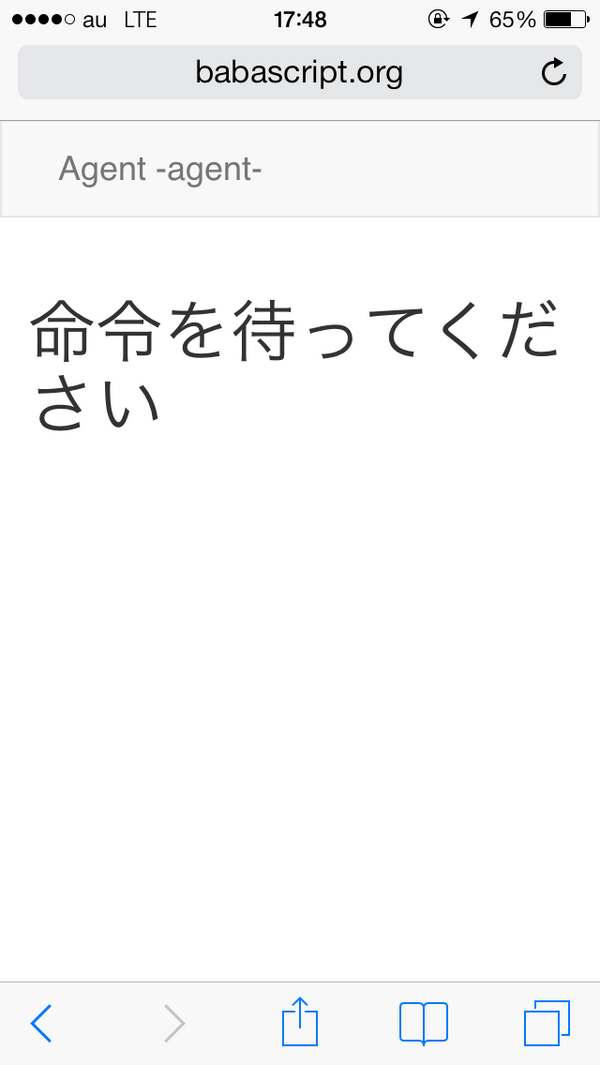
\includegraphics[width=45mm, bb= 0 0 600 1065]{images/image4.png}
    }
    \caption{待機時の画面}
    \label{babascript-wait}
  \end{center}
\end{figure}
\begin{figure}[tb]
  \begin{center}
    \fbox{
      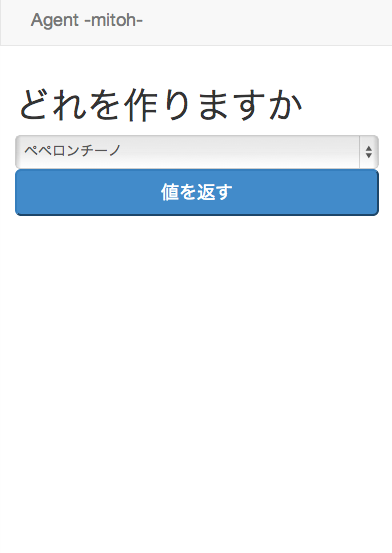
\includegraphics[width=45mm, bb= 0 0 392 553]{images/babascript-list.png}
    }
    \caption{リスト表示時の画面}
    \label{babascript-list}
  \end{center}
\end{figure}



\section{応用例}
\subsection{人の仕事や役割をプログラム化する}
人の行動をプログラムとして記述可能になることで、人の仕事や役割がプログラム化・実行可能となる。
仕事や役割はマニュアルやドキュメントという形で言語化されていることが多い。
これらのマニュアル・ドキュメントをプログラム化し、実行できるようになれば、人はプログラムからの命令に従うだけで様々な仕事や役割を達成することができるようになる。
ただ命令に従うだけなので、経験・引き継ぎは必要なく、人の代替が容易となる。
また、全ての仕事はプログラムから管理されるため、人の運用効率の数値化などが可能となる。


\subsection{柔軟な実世界プログラミング}
人をセンサーやアクチュエータとして利用することで、現在一般的に使われているセンサーやアクチュエータでは実現困難な実世界プログラミングが可能となる。
現在のセンサー技術では、その場の雰囲気を数値化・文字列化するなどのコンテキスト情報をうまく扱うことはとても難しい。
また、アクチュエータも単一の動きに特化したものが多く、複雑な動きを実現することは難しい。
BabaScript環境でならば、プログラム上で人はセンサーやアクチュエータのオブジェクトと類似の挙動をすることができる。

また、人とセンサ・アクチュエータをうまく使い分けていくことが可能となる。
コンテキスト情報を扱いそうなら人に、温度などの数値を取得するだけならばセンサーを使うとことができる。
センサー・アクチュエータがその場に存在するならばセンサー・アクチュエータを動作させるが、ない場合は人に命令する、といったことも実現可能である。


\section{関連研究}
計算機では処理できないようなタスクを解決するために、人を計算資源としてプログラムに組み込む手法はヒューマンコンピュテーション\cite{humancomputation}と呼ばれ、様々な研究が行われている。
米Amazonが運営している AmazonMechanicalTurk\cite{amt} は、クラウドソーシングのためのプラットフォームだ。
mTurk API を通し、人間に対してタスクの実行を依頼することができる。
AUTOMAN\cite{automan}は、crowdprogrammingという概念を唱え、通常のプログラミング言語内でコンピュータによる計算と人による計算を統合した。
CrowdForge\cite{crowdforge}は、MapReduceのような機能をクラウドソーシングのためのフレームワークだ。
クラウドソーシングするタスクを適切に分割し、人力で解かせた後、集合させるといったことができる。
jabberwocky\cite{jabberwocky}は、クラウドソーシングプラットフォームを自由に作れる・再利用できる仕組みをもったDormouseやMapReduce的に人リソースを扱えるManReduce、SQL風のスクリプト言語Dogから構成される、クラウドソーシングのためのフレームワークだ。
CrowdDB\cite{crowddb}では機械だけでは答えられないようなDBへのクエリに対し、クラウドソーシングを使うことで返答させるためのSQLライクなプログラミングを提案している。
CyLog\cite{cylog}はDatalogに似たヒューマンコンピュテーションのためのプログラミング言語だ。
人をデータソースとしてプログラムの中で利用する手法を提案している。
これらの研究は、人を計算資源・データソースとして捉え、コンピュータの代替として人を利用している。
本研究では、人の行動そのものをプログラムとして記述し、実行可能なものにすることを目的としている。

ユビキタスコンピューティングの研究分野においては、Human as Sensor といった概念も存在しており、研究が行われている。
MoboQ\cite{moboq}では、場所ベースのQ\&Aサービスを実装し、その効果を検証した。
Moboqではプラットフォームとしてソーシャルメディアを利用しており、ソーシャルメディア上の人たちをセンサーとして利用している。
スマートフォンを使ったセンシングのためのプラットフォームとしては、PRISM\cite{prism}などが発表されている。
これらの研究では、人をセンサーとして利用し、情報を収集することを目的としている。
本研究では、人の行動をプログラムとして記述することを目的としており、その利用方法はセンサーに限定されたものではない。

人のワークフローを定義するWebサービスとしては、atled\cite{atled}やQuestetra\cite{questetra}などが存在するが、これらのサービスは、人の行動をプログラムで記述するものではない。
BabaScript環境では、人・コンピュータの動作を同一のプログラム上で記述することが可能だ。

\section{おわりに}
\subsection{今後の課題}
今後は以下の問題について検討する。
\subsubsection{命令に対する実行保証性}
プログラムからの命令を人が必ず実行するとは限らない。
命令が表示されるデバイスを見ていないことや、そもそも命令を無視するといったことも考えられる。
今後検討していく。

\subsection{結論}
本論文では、人の行動を記述可能なプログラミング環境 BabaScript を提案した。
人力処理構文と命令を受け取り値を返すことのできるクライアントアプリケーションを組み合わせることによって、プログラム上で人を表現することが可能になった。
BabaScript環境においては、人とコンピュータの双方は同じプログラム内で動きを定義することができる。
今後は、課題の解決と有用性の検証を行う。

\vspace{5mm}

\begin{thebibliography}{99}
\bibitem{humancomputation}
L. von Ahn. 2007. Human computation. In Proceedings of the 4th international conference on Knowledge capture. K-CAP '07. ACM.
\bibitem{amt}
Amazon Machanical Turk
http://www.mturk.com
\bibitem{automan}
Barowy, D. W., Curtsinger, C., Berger, E. D., andMcGregor, A. AutoMan: A Platform for Integrating Human-Based and DigitalComputation. In Proc. OOPSLA (2012).
\bibitem{crowdforge}
A. Kittur, B. Smus, and R. E. Kraut. CrowdForge: Crowdsourc- ing Complex Work. Tech. Rep. CMU-HCII-11-100, Human- Computer Interaction Institute, School of Computer Science, Carnegie Mellon University, February 2011.
\bibitem{jabberwocky}
S. Ahmad, A. Battle, Z. Malkani, and S. Kamvar. The Jabberwocky Programming Environment for Structured Social Computing. In UIST, pp. 53–64, 2011.
\bibitem{crowddb}
M. J. Franklin, D. Kossmann, T. Kraska, S. Ramesh, and R. Xin. CrowdDB: Answering Queries with Crowdsourcing. In SIGMOD, pp. 61–72, 2011.
\bibitem{cylog}
Atsuyuki Morishima, Norihide Shinagawa, Tomomi Mitsuishi, Hideto Aoki, Shun Fukusumi. “CyLog/Crowd4U: A Declarative Platform for Complex Data-centric"
\bibitem{moboq}
Liu, Yefeng and Alexandrova, Todorka and Nakajima, Tatsuo. Using Stranger As Sensors: Temporal and Geo-sensitive Question Answering via Social Media. Proceedings of the 22Nd International Conference on World Wide Web, pp. 803--814, 2013
\bibitem{prism}
Das, Tathagata and Mohan, Prashanth and Padmanabhan, Venkata N. and Ramjee, Ramachandran and Sharma, Asankhaya. PRISM: Platform for Remote Sensing Using Smartphones. Proceedings of the 8th International Conference on Mobile Systems, Applications, and Services. pp.63--76, 2010.
\bibitem{atled}
https://www.atled.jp/
\bibitem{questetra}
http://www.questetra.com/
\end{thebibliography}


\end{document}
